\documentclass[10pt,aspectratio=169]{beamer}
\usetheme{metropolis}

\usepackage[T1]{fontenc}
\usepackage[utf8]{inputenc}
\usepackage{amsmath,amssymb}
\usepackage{booktabs}
\usepackage{tikz}
\usepackage{pgfplots}
\pgfplotsset{compat=1.18}
\usetikzlibrary{positioning,arrows.meta,shapes.geometric,calc,backgrounds,fit}
\usepackage{appendixnumberbeamer}

% ---- paleta ----
\definecolor{cblue}{HTML}{3B7DD8}
\definecolor{cred}{HTML}{C0392B}
\definecolor{cgreen}{HTML}{2E8B57}
\definecolor{corange}{HTML}{E8833A}
\definecolor{cgray}{HTML}{6B6B6B}
\setbeamercolor{frametitle}{bg=cblue!90!black}

% ---- estilos tikz/pgf reutilizáveis ----
\tikzset{
  block/.style={draw, rounded corners, thick, minimum height=1cm, minimum width=2cm, align=center, font=\small},
  sig/.style={-{Latex[length=2mm]}, thick},
  mod/.style={draw, rounded corners, thick, fill=cblue!8, align=center, font=\scriptsize, minimum width=2.6cm, minimum height=0.9cm},
}
\pgfplotsset{
  scatterstyle/.style={only marks, mark=*, mark size=0.45pt},
  myaxis/.style={width=\linewidth, height=4.2cm, grid=both, grid style={gray!20},
                 tick label style={font=\tiny}, label style={font=\scriptsize},
                 title style={font=\scriptsize\bfseries}, legend style={font=\tiny}},
}

% ---- coloração da equação NARX ----
\newcommand{\offsetcol}[1]{\textcolor{cgray}{#1}}
\newcommand{\arcol}[1]{\textcolor{cblue}{#1}}
\newcommand{\nlcol}[1]{\textcolor{cred}{#1}}

\title{Identificação e Linearização de um Amplificador de Potência de RF}
\subtitle{Modelo NARX com refinamento por Algoritmo Genético}
\author{Isaac Kosloski}
\institute{Grupo de Pesquisa --- Mestrado}
\date{\today}

\begin{document}

\maketitle

\begin{frame}{Roteiro}
  \tableofcontents
\end{frame}

% =====================================================================
\section{O problema: não-linearidade do PA}
% =====================================================================
\begin{frame}{O amplificador de potência: ideal vs. real}
  \begin{center}
  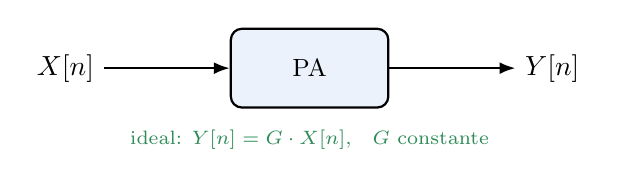
\begin{tikzpicture}[node distance=1.6cm]
    \node (x) {$X[n]$};
    \node[block, right=of x, fill=cblue!10] (pa) {PA};
    \node[right=of pa] (y) {$Y[n]$};
    \draw[sig] (x) -- (pa);
    \draw[sig] (pa) -- (y);
    \node[below=0.15cm of pa, font=\scriptsize, text=cgreen] {ideal: $Y[n]=G\cdot X[n]$, \; $G$ constante};
  \end{tikzpicture}
  \end{center}
  \vspace{0.3cm}
  Perto da saturação --- onde o PA é \alert{eficiente} --- quatro efeitos quebram a idealidade:
  \begin{columns}[T]
    \column{0.5\textwidth}
    \begin{itemize}\setlength\itemsep{2pt}
      \item \textbf{AM-AM}: ganho cai com a amplitude (compressão)
      \item \textbf{AM-PM}: fase gira com a amplitude
    \end{itemize}
    \column{0.5\textwidth}
    \begin{itemize}\setlength\itemsep{2pt}
      \item \textbf{IM3}: intermodulação cúbica $\Rightarrow$ \emph{spectral regrowth}
      \item \textbf{Memória}: a saída depende do passado
    \end{itemize}
  \end{columns}
  \vspace{0.2cm}
  \begin{alertblock}{\footnotesize Trade-off fundamental}
    \footnotesize Eficiência cresce perto da saturação; linearidade se perde lá. Linearizar = ter as duas.
  \end{alertblock}
\end{frame}

% =====================================================================
\section{Representação do sinal (I/Q)}
% =====================================================================
\begin{frame}{Banda-base complexa --- I/Q}
  \begin{columns}[c]
    \column{0.52\textwidth}
    Sinal de RF: $s(t)=\mathrm{Re}\{x(t)e^{j\omega t}\}$.\\[2pt]
    Modelamos o \alert{envelope complexo} $x(t)$:
    \[ X[n]=X_r + jX_i,\quad |X|=\text{amplitude},\ \angle X=\text{fase} \]
    Dados: 4 colunas reais por amostra
    ($X_r,X_i,Y_r,Y_i$), $48{,}384$ amostras.
    \column{0.48\textwidth}
    \begin{tikzpicture}
      \begin{axis}[myaxis, title={Entrada $X[n]$ (referência)},
          xlabel={$I$}, ylabel={$Q$}, axis equal image, height=4.4cm]
        \addplot[scatterstyle, color=cblue, opacity=0.5]
          table[x=i,y=q,col sep=comma]{data/const_in.csv};
      \end{axis}
    \end{tikzpicture}
  \end{columns}
\end{frame}

% =====================================================================
\section{O modelo NARX}
% =====================================================================
\begin{frame}{Estrutura NARX}
  \emph{Nonlinear AutoRegressive with eXogenous inputs}
  \vspace{0.4cm}
  \[
    Y(t)=\offsetcol{\underbrace{c}_{\text{offset DC}}}
    +\arcol{\underbrace{A_1 Y(t{-}1)+A_2 Y(t{-}2)}_{\text{memória autorregressiva}}}
    +\nlcol{\underbrace{\textstyle\sum_k \beta_k\,\phi_k(X(t),X(t{-}1),X(t{-}2))}_{\text{regressores polinomiais (não-linear)}}}
  \]
  \vspace{0.3cm}
  \begin{itemize}\setlength\itemsep{3pt}
    \item Base: $X_r^{d}$ e $X_i^{d}$, com $d\in\{1,2,3\}$ e atrasos $\{0,1,2\}$
    \item $2\times3\times3 = \mathbf{18}$ regressores $\phi$ $\;\times\;2$ saídas $=\mathbf{36}$ coeficientes $\beta$
    \item $d{=}1$: ganho nominal \;|\; $d{=}2$: HD2/IM2 \;|\; $d{=}3$: AM-AM, AM-PM, IM3
  \end{itemize}
\end{frame}

\begin{frame}{A equação identificada --- lendo a física}
  \footnotesize
  \[
  \begin{aligned}
    Y_r(t) &\approx \arcol{+23{,}457\,X_r} \arcol{-1{,}474\,X_i}
            \;\nlcol{-0{,}463\,X_r^3} \nlcol{+2{,}042\,X_i^3} \;+\; (\text{memória}\approx 0)\\
    Y_i(t) &\approx \arcol{+1{,}475\,X_r} \arcol{+23{,}457\,X_i}
            \;\nlcol{-2{,}043\,X_r^3} \nlcol{-0{,}467\,X_i^3} \;+\; (\text{memória}\approx 0)
  \end{aligned}
  \]
  \normalsize
  \begin{enumerate}\setlength\itemsep{3pt}
    \item Parte linear $=$ matriz de \textbf{ganho + rotação}: $|G|\approx 23{,}46$ (27{,}4~dB), $\theta\approx 3{,}6^\circ$
    \item Coeficientes AR e de atraso $\sim 10^{-5}$ $\Rightarrow$ \textbf{memória desprezível} (quase estático)
    \item Distorção dominada pelos termos \textbf{cúbicos}
  \end{enumerate}
\end{frame}

% =====================================================================
\section{Identificação: o papel do Algoritmo Genético}
% =====================================================================
\begin{frame}{Por que GA? \emph{Equation-error} vs. \emph{output-error}}
  \begin{columns}[T]
    \column{0.5\textwidth}
    \centering\scriptsize \textbf{Equation-error} (LS é ótimo)\\[4pt]
    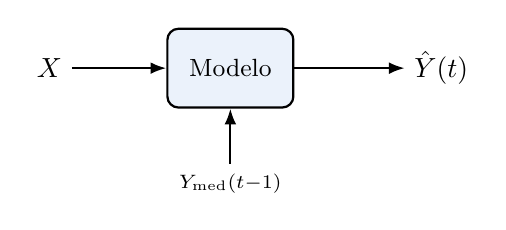
\begin{tikzpicture}[node distance=0.9cm and 1.2cm]
      \node (x) {$X$}; \node[block, right=of x, fill=cblue!10, minimum width=1.6cm] (m) {Modelo};
      \node[right=1.4cm of m] (yh) {$\hat Y(t)$};
      \node[below=0.7cm of m, font=\scriptsize] (ym) {$Y_{\text{med}}(t{-}1)$};
      \draw[sig] (x) -- (m); \draw[sig] (m) -- (yh);
      \draw[sig] (ym) -- (m);
    \end{tikzpicture}\\[3pt]
    \scriptsize realimenta a saída \emph{medida} $\Rightarrow$ linear nos parâmetros
    \column{0.5\textwidth}
    \centering\scriptsize \textbf{Output-error} (não-convexo)\\[4pt]
    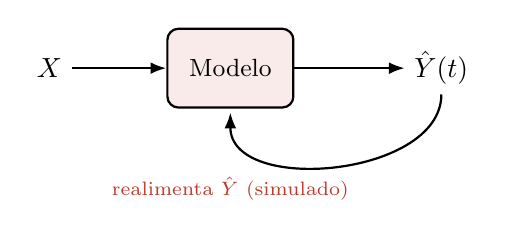
\begin{tikzpicture}[node distance=0.9cm and 1.2cm]
      \node (x) {$X$}; \node[block, right=of x, fill=cred!10, minimum width=1.6cm] (m) {Modelo};
      \node[right=1.4cm of m] (yh) {$\hat Y(t)$};
      \draw[sig] (x) -- (m); \draw[sig] (m) -- (yh);
      \draw[sig] (yh) to[out=-90,in=-90] ($(m.south)+(0,-0.05)$);
      \node[below=0.75cm of m, font=\scriptsize, text=cred] {realimenta $\hat Y$ (simulado)};
    \end{tikzpicture}\\[3pt]
    \scriptsize a recursão torna o custo \alert{não-convexo}
  \end{columns}
  \vspace{0.3cm}
  \footnotesize O modelo roda \textbf{recursivamente} (simulação) $\Rightarrow$ LS puro não se aplica.
  O \textbf{GA} é global, sem gradiente, e refina a semente em modo output-error.
\end{frame}

\begin{frame}{De onde vem a semente: linhagem VARMAX $\to$ NARX}
  \begin{center}
  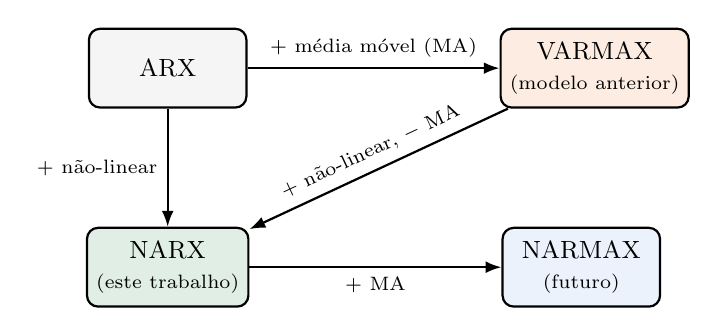
\begin{tikzpicture}[node distance=1.5cm and 3.2cm]
    \node[block, fill=gray!8] (arx) {ARX};
    \node[block, right=of arx, fill=corange!15] (armax) {VARMAX\\\scriptsize(modelo anterior)};
    \node[block, below=of arx, fill=cgreen!15] (narx) {NARX\\\scriptsize(este trabalho)};
    \node[block, right=of narx, fill=cblue!10] (narmax) {NARMAX\\\scriptsize(futuro)};
    \draw[sig] (arx) -- node[above,font=\scriptsize]{$+$ média móvel (MA)} (armax);
    \draw[sig] (arx) -- node[left,font=\scriptsize]{$+$ não-linear} (narx);
    \draw[sig] (narx) -- node[below,font=\scriptsize]{$+$ MA} (narmax);
    \draw[sig] (armax) -- node[sloped,above,font=\scriptsize]{$+$ não-linear, $-$ MA} (narx);
  \end{tikzpicture}
  \end{center}
  \footnotesize
  Aluno anterior: \textbf{VARMAX} (vetorial I/Q, com MA) $+$ termos não-lineares.\\
  Implantado: \textbf{NARX} (sem MA). Na simulação $X{\to}Y$ as inovações entram com média
  zero $\Rightarrow$ o MA não contribui. O fecho natural é o \textbf{NARMAX}.
\end{frame}

% =====================================================================
\section{O Algoritmo Genético}
% =====================================================================
\begin{frame}{O laço evolutivo}
  \begin{columns}[c]
    \column{0.54\textwidth}
    \centering
    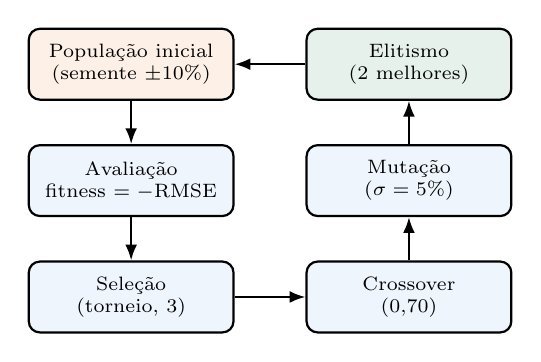
\begin{tikzpicture}[node distance=0.55cm and 0.9cm, every node/.style={font=\scriptsize}]
      \node[mod, fill=corange!12] (init) {População inicial\\(semente $\pm10\%$)};
      \node[mod, below=of init] (eval) {Avaliação\\ fitness $=-$RMSE};
      \node[mod, below=of eval] (sel) {Seleção\\(torneio, 3)};
      \node[mod, right=of sel] (cx) {Crossover\\(0{,}70)};
      \node[mod, right=of eval] (mut) {Mutação\\($\sigma=5\%$)};
      \node[mod, right=of init, fill=cgreen!12] (eli) {Elitismo\\(2 melhores)};
      \draw[sig] (init) -- (eval);
      \draw[sig] (eval) -- (sel);
      \draw[sig] (sel) -- (cx);
      \draw[sig] (cx) -- (mut);
      \draw[sig] (mut) -- (eli);
      \draw[sig] (eli) -- (init);
    \end{tikzpicture}
    \column{0.46\textwidth}
    \scriptsize
    \begin{tabular}{@{}ll@{}}
      \toprule
      Parâmetro & Valor\\
      \midrule
      População & 50 \\
      Gerações & 100 \\
      Crossover & 0{,}70 \\
      Mutação & 0{,}20 ($\sigma_{\text{rel}}=5\%$) \\
      Torneio & 3 \\
      Elites & 2 \\
      Perturbação inicial & $\pm10\%$ \\
      Semente aleatória & 42 \\
      \bottomrule
    \end{tabular}\\[4pt]
    Cromossomo $=$ vetor dos 36 $\beta$.\\
    Biblioteca: \textbf{DEAP}.
  \end{columns}
\end{frame}

% =====================================================================
\section{Arquitetura do software}
% =====================================================================
\begin{frame}{Arquitetura --- separação de responsabilidades}
  \begin{center}
  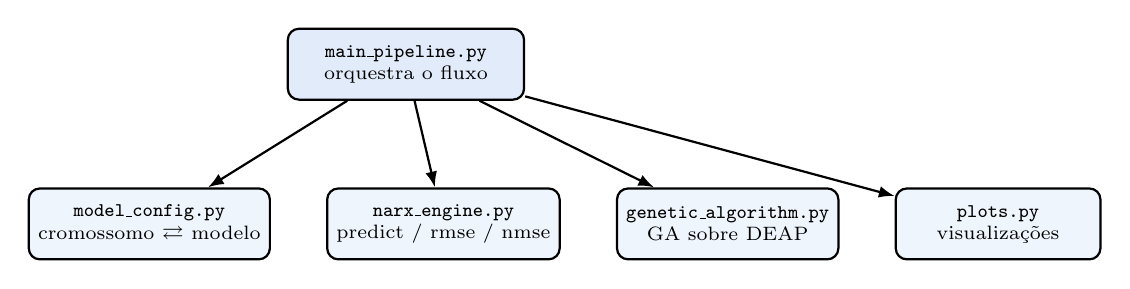
\begin{tikzpicture}[node distance=0.5cm and 0.7cm]
    \node[mod, fill=cblue!15, minimum width=3cm] (main) {\texttt{main\_pipeline.py}\\orquestra o fluxo};
    \node[mod, below left=1.1cm and 0.2cm of main] (cfg) {\texttt{model\_config.py}\\cromossomo $\rightleftarrows$ modelo};
    \node[mod, right=of cfg] (eng) {\texttt{narx\_engine.py}\\predict / rmse / nmse};
    \node[mod, right=of eng] (ga) {\texttt{genetic\_algorithm.py}\\GA sobre DEAP};
    \node[mod, right=of ga] (plt) {\texttt{plots.py}\\visualizações};
    \draw[sig] (main) -- (cfg); \draw[sig] (main) -- (eng);
    \draw[sig] (main) -- (ga);  \draw[sig] (main) -- (plt);
  \end{tikzpicture}
  \end{center}
  \footnotesize
  O motor NARX não conhece o GA; o GA não conhece física de PA. A fronteira é a tradução
  cromossomo $\rightleftarrows$ modelo $\Rightarrow$ dá para trocar o otimizador mexendo num módulo só.
\end{frame}

% =====================================================================
\section{Métricas}
% =====================================================================
\begin{frame}{Métricas de avaliação}
  \scriptsize
  \begin{tabular}{@{}lll@{}}
    \toprule
    Métrica & Mede & Referência (3GPP/indústria)\\
    \midrule
    RMSE & erro absoluto (resíduo complexo) & comparar vs.\ semente\\
    NMSE & erro normalizado pela potência (dB) & BOM $<-30$~dB \\
    EVM & erro relativo da constelação (\%) & BOM $<3{,}5\%$ (256-QAM)\\
    $|G|$ std & planicidade do ganho & BOM $<0{,}5$~dB\\
    $\angle G$ std & planicidade da fase & BOM $<2{,}0^\circ$\\
    \bottomrule
  \end{tabular}
  \vspace{0.4cm}
  \normalsize
  \begin{block}{\footnotesize Identidade útil}
    \footnotesize $\text{EVM}=10^{\,\text{NMSE}_{\text{dB}}/20}$.\quad
    Confira: $-27{,}82~\text{dB}\Rightarrow 10^{-27{,}82/20}=4{,}06\%$.
  \end{block}
\end{frame}

% =====================================================================
\section{Resultados}
% =====================================================================
\begin{frame}{Resultados --- números reais}
  \footnotesize
  \begin{tabular}{@{}lll@{}}
    \toprule
    Métrica & Valor & Veredito\\
    \midrule
    Amostras & $48{,}384$ & ---\\
    RMSE & $0{,}74771$ & melhor do GA\\
    NMSE & $-27{,}82$~dB & \textcolor{corange}{a melhorar}\\
    EVM & $4{,}06\%$ & \textcolor{corange}{a melhorar}\\
    Ganho médio & $27{,}40$~dB & \textcolor{cgreen}{esperado}\\
    Planicidade ganho (std) & $0{,}223$~dB & \textcolor{cgreen}{BOM}\\
    Planicidade fase (std) & $4{,}763^\circ$ & \textcolor{corange}{a melhorar}\\
    \bottomrule
  \end{tabular}
  \vspace{0.3cm}\\
  \footnotesize Fidelidade \textbf{moderada}: ótima em ganho, abaixo da meta em NMSE, EVM e fase.
\end{frame}

\begin{frame}{Caracterização: AM-AM e AM-PM (medido vs.\ previsto)}
  \begin{columns}[c]
    \column{0.5\textwidth}
    \begin{tikzpicture}
      \begin{axis}[myaxis, title={AM-AM --- ganho (dB)},
          xlabel={$|X[n]|$}, ylabel={$|Y|/|X|$ (dB)}, enlargelimits=0.03]
        \addplot[scatterstyle, color=cblue, opacity=0.5] table[x=xmag,y=gm,col sep=comma]{data/amam.csv};
        \addplot[scatterstyle, color=cred,  opacity=0.5] table[x=xmag,y=go,col sep=comma]{data/amam.csv};
        \legend{Medido, Previsto}
      \end{axis}
    \end{tikzpicture}
    \column{0.5\textwidth}
    \begin{tikzpicture}
      \begin{axis}[myaxis, title={AM-PM --- fase (graus)},
          xlabel={$|X[n]|$}, ylabel={$\angle Y-\angle X$}, enlargelimits=0.03]
        \addplot[scatterstyle, color=cblue, opacity=0.5] table[x=xmag,y=pm,col sep=comma]{data/ampm.csv};
        \addplot[scatterstyle, color=cred,  opacity=0.5] table[x=xmag,y=po,col sep=comma]{data/ampm.csv};
        \draw[dashed, gray] ({rel axis cs:0,0}|-{axis cs:0,0}) -- ({rel axis cs:1,0}|-{axis cs:0,0});
        \legend{Medido, Previsto}
      \end{axis}
    \end{tikzpicture}
  \end{columns}
  \footnotesize Ganho cai $\sim$1~dB (compressão, std $0{,}223$~dB). Fase parte de $\sim$3{,}6$^\circ$ e varre até $-3^\circ$ (std $4{,}76^\circ$, o pior indicador).
\end{frame}

\begin{frame}{Constelação IQ --- entrada, medido, previsto}
  \begin{columns}[c]
    \column{0.34\textwidth}
    \begin{tikzpicture}
      \begin{axis}[myaxis, title={Entrada}, axis equal image, height=3.8cm, xlabel={$I$}, ylabel={$Q$}]
        \addplot[scatterstyle, color=cblue, opacity=0.5] table[x=i,y=q,col sep=comma]{data/const_in.csv};
      \end{axis}
    \end{tikzpicture}
    \column{0.34\textwidth}
    \begin{tikzpicture}
      \begin{axis}[myaxis, title={Medido}, axis equal image, height=3.8cm, xlabel={$I$}]
        \addplot[scatterstyle, color=cblue, opacity=0.5] table[x=i,y=q,col sep=comma]{data/const_meas.csv};
      \end{axis}
    \end{tikzpicture}
    \column{0.34\textwidth}
    \begin{tikzpicture}
      \begin{axis}[myaxis, title={Previsto (GA)}, axis equal image, height=3.8cm, xlabel={$I$}]
        \addplot[scatterstyle, color=cgreen, opacity=0.5] table[x=i,y=q,col sep=comma]{data/const_pred.csv};
      \end{axis}
    \end{tikzpicture}
  \end{columns}
  \footnotesize Saída amplificada $\sim$23$\times$ (eixo $\pm$30 vs.\ $\pm$1{,}2). O modelo reproduz a constelação medida; o erro de $\sim$4\% de EVM não é visível nesta escala.
\end{frame}

\begin{frame}{Erro por amostra e melhora do GA}
  \begin{columns}[c]
    \column{0.62\textwidth}
    \begin{tikzpicture}
      \begin{axis}[myaxis, title={Erro absoluto $|Y_{\text{med}}-Y_{\text{prev}}|$},
          xlabel={amostra}, ylabel={erro}, height=4.4cm, ymin=0]
        \addplot[mark=none, color=corange, line width=0.2pt] table[x=n,y=e,col sep=comma]{data/error.csv};
      \end{axis}
    \end{tikzpicture}
    \column{0.38\textwidth}
    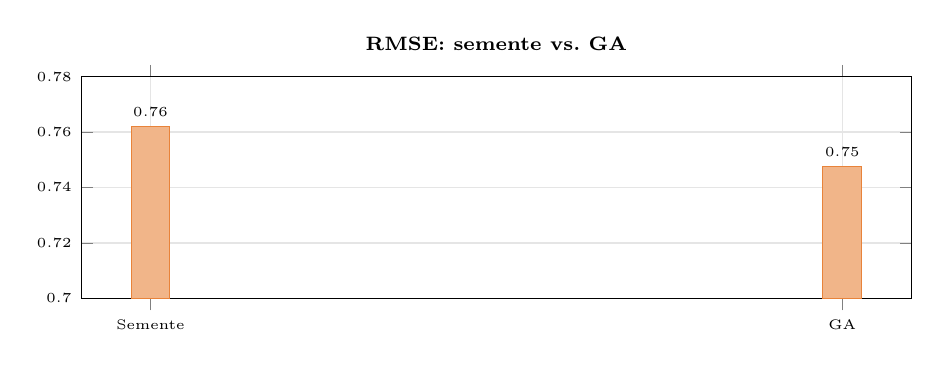
\begin{tikzpicture}
      \begin{axis}[myaxis, title={RMSE: semente vs.\ GA}, height=4.4cm,
          ybar, symbolic x coords={Semente,GA}, xtick=data, bar width=14pt,
          ymin=0.7, ymax=0.78, nodes near coords, nodes near coords style={font=\tiny}]
        \addplot[fill=corange!60, draw=corange] coordinates {(Semente,0.76203) (GA,0.74771)};
      \end{axis}
    \end{tikzpicture}
  \end{columns}
  \footnotesize O resíduo tem \textbf{estrutura periódica} (não é branco) $\Rightarrow$ subajuste da não-linearidade nos picos, \emph{não} overfitting. GA melhora só $1{,}9\%$ (semente já era boa).
\end{frame}

\begin{frame}{Convergência do GA --- leitura honesta}
  \begin{columns}[c]
    \column{0.62\textwidth}
    
\includegraphics[width=\linewidth]{figs/ga_convergence.png}
    \column{0.38\textwidth}
    \footnotesize
    \begin{itemize}\setlength\itemsep{4pt}
      \item Verde (elite) quase \textbf{plano}: $0{,}762\to0{,}7477$
      \item Azul (média) flutua: população \textbf{explora} sem achar nada melhor
      \item Elitismo $\Rightarrow$ melhor nunca piora
    \end{itemize}
    \alert{Não é falha:} a semente VARMAX já estava perto de um ótimo local. Ganhos exigem mudar a \emph{estrutura}, não mais gerações.
  \end{columns}
\end{frame}

% =====================================================================
\section{A linearização: $X\cdot G = Y$}
% =====================================================================
\begin{frame}{O ganho linearizado}
  \begin{columns}[c]
    \column{0.55\textwidth}
    Ganho complexo por amostra:
    \[ G[n]=\frac{Y_{\text{opt}}[n]}{X[n]} \]
    Ganho médio (escalar complexo):
    \[ \overline{G}=\langle G[n]\rangle \approx 23{,}46\,\angle\,3{,}6^\circ \]
    Relação linearizada entregue:
    \[ \boxed{\,X[n]\cdot \overline{G}\approx Y[n]\,} \]
    \column{0.45\textwidth}
    \footnotesize
    \begin{itemize}\setlength\itemsep{4pt}
      \item $G[n]$ \emph{varia} com a amplitude $\Rightarrow$ é o próprio AM-AM/AM-PM
      \item $\overline{G}$ é a referência \textbf{linear} ideal
      \item Próximo passo: \textbf{DPD} aplica $G^{-1}$ antes do PA
    \end{itemize}
    \vspace{0.2cm}
    Este trabalho \textbf{identifica} o PA e caracteriza $\overline{G}$: pré-requisito da pré-distorção.
  \end{columns}
\end{frame}

% =====================================================================
\section{Limitações e trabalhos futuros}
% =====================================================================
\begin{frame}{A maior limitação: quebra de simetria rotacional}
  \begin{columns}[c]
    \column{0.5\textwidth}
    \begin{tikzpicture}
      \begin{axis}[myaxis, title={Ganho vs.\ \emph{ângulo} de X ($|X|$ fixo)},
          xlabel={$\angle X$ (graus)}, ylabel={ganho (dB)}, xmin=0, xmax=360,
          xtick={0,90,180,270,360}, height=4.2cm]
        \addplot[mark=none, color=cgreen, thick] table[x=ang,y=g03,col sep=comma]{data/rot.csv};
        \addplot[mark=none, color=cblue,  thick] table[x=ang,y=g06,col sep=comma]{data/rot.csv};
        \addplot[mark=none, color=corange, thick] table[x=ang,y=g10,col sep=comma]{data/rot.csv};
        \addplot[mark=none, color=cred,    thick] table[x=ang,y=g115,col sep=comma]{data/rot.csv};
        \addplot[dashed, gray] coordinates {(0,27.405)(360,27.405)};
        \legend{0{,}3,0{,}6,1{,}0,1{,}15}
      \end{axis}
    \end{tikzpicture}
    \column{0.5\textwidth}
    \begin{tikzpicture}
      \begin{axis}[myaxis, title={Fase vs.\ \emph{ângulo} de X ($|X|$ fixo)},
          xlabel={$\angle X$ (graus)}, ylabel={fase (graus)}, xmin=0, xmax=360,
          xtick={0,90,180,270,360}, height=4.2cm]
        \addplot[mark=none, color=cgreen, thick] table[x=ang,y=p03,col sep=comma]{data/rot.csv};
        \addplot[mark=none, color=cblue,  thick] table[x=ang,y=p06,col sep=comma]{data/rot.csv};
        \addplot[mark=none, color=corange, thick] table[x=ang,y=p10,col sep=comma]{data/rot.csv};
        \addplot[mark=none, color=cred,    thick] table[x=ang,y=p115,col sep=comma]{data/rot.csv};
        \addplot[dashed, gray] coordinates {(0,0)(360,0)};
        \legend{0{,}3,0{,}6,1{,}0,1{,}15}
      \end{axis}
    \end{tikzpicture}
  \end{columns}
  \footnotesize A amplitude fixa, ganho/fase variam só com o ângulo (até $0{,}53$~dB e $3{,}5^\circ$) --- um PA físico daria retas. Artefato da base $X_r^d,X_i^d$ (não covariante à fase).
\end{frame}

\begin{frame}{Trabalhos futuros}
  \begin{enumerate}\setlength\itemsep{5pt}
    \item \textbf{Base de regressores}: migrar de $X_r^d,X_i^d$ para o \emph{memory polynomial} $x\cdot|x|^{2k}$ (covariante à fase) $\Rightarrow$ deve corrigir a planicidade de fase.
    \item \textbf{Validação treino/teste}: hoje as métricas são no conjunto de ajuste; reportar NMSE/EVM em dados não vistos.
    \item \textbf{Baseline}: comparar GA vs.\ semente VARMAX pura vs.\ LS direto.
    \item \textbf{NARMAX}: reincorporar o termo MA para o resíduo colorido.
    \item \textbf{DPD}: fechar o ciclo com a pré-distorção digital.
  \end{enumerate}
\end{frame}

% =====================================================================
\section{Conclusão}
% =====================================================================
\begin{frame}{Conclusão}
  \begin{itemize}\setlength\itemsep{5pt}
    \item NARX identifica os efeitos não-lineares do PA numa só equação.
    \item A equação revela: ganho $27{,}4$~dB $+$ rotação $3{,}6^\circ$ $+$ cúbica dominante $+$ memória fraca.
    \item GA refinou um modelo VARMAX prévio ($0{,}762\to0{,}7477$).
    \item Fidelidade moderada: ganho plano (bom); NMSE/EVM/fase a melhorar.
    \item Ponto forte: o \textbf{diagnóstico} é claro $\Rightarrow$ próximos passos definidos.
  \end{itemize}
  \vspace{0.4cm}
  \begin{center}\large Obrigado! \quad \small (perguntas)\end{center}
\end{frame}

\appendix
\begin{frame}{Backup --- linearização $|Y|$ vs $|X|$}
  \begin{columns}[c]
    \column{0.55\textwidth}
    \begin{tikzpicture}
      \begin{axis}[myaxis, title={$|Y|$ vs $|X|$ (escala esconde a compressão)},
          xlabel={$|X[n]|$}, ylabel={$|Y[n]|$}, height=4.6cm]
        \addplot[scatterstyle, color=cgreen, opacity=0.5]
          table[x expr=\thisrow{xmag}, y expr=\thisrow{xmag}*23.456, col sep=comma]{data/amam.csv};
      \end{axis}
    \end{tikzpicture}
    \column{0.45\textwidth}
    \footnotesize Numa escala $0$--$27$, a compressão de $\pm0{,}5$~dB é invisível: parece uma reta perfeita. A caracterização real exige o gráfico de \emph{ganho} ampliado (slide de AM-AM).
  \end{columns}
\end{frame}

\begin{frame}{Backup --- identidades e referências}
  \footnotesize
  \begin{itemize}\setlength\itemsep{4pt}
    \item $\text{EVM}=10^{\text{NMSE}_{\text{dB}}/20}$;\quad rotação estática $\theta=\arctan(1{,}4743/23{,}4565)\approx3{,}6^\circ$
    \item Volterra (Schetzen, 1980); Memory Polynomial / GMP (Morgan et al., 2006)
    \item NARMAX (Leontaritis \& Billings, 1985)
    \item Lóbulos $\propto$ 3$^\circ$ harmônico angular: $\cos^3\theta=\tfrac{3\cos\theta+\cos3\theta}{4}$
  \end{itemize}
\end{frame}

\end{document}
